\documentclass[11pt,a4paper]{article}

\usepackage[margin=2.1cm]{geometry}
\usepackage[T1]{fontenc}
\usepackage[utf8]{inputenc}
\usepackage{lmodern}
\usepackage{microtype}
\usepackage{amsmath,amssymb,mathtools}
\usepackage{booktabs,array,tabularx}
\usepackage{graphicx}
\usepackage{xcolor}
\usepackage{tcolorbox}
\tcbuselibrary{skins,breakable}
\usepackage{fancyhdr}
\usepackage{hyperref}
\usepackage{enumitem}

\definecolor{navy}{HTML}{1B365D}
\definecolor{slate}{HTML}{2C5282}
\definecolor{tint}{HTML}{F4F7FA}
\definecolor{amber}{HTML}{8A5A00}
\definecolor{ambertint}{HTML}{FFFBEB}
\definecolor{greenink}{HTML}{1E5631}
\definecolor{greentint}{HTML}{F1F8F4}
\definecolor{crimson}{HTML}{9B2C2C}
\definecolor{crimsontint}{HTML}{FFF5F5}

\hypersetup{
  colorlinks=true,
  linkcolor=slate,
  urlcolor=slate,
  pdftitle={Independent Verification and Audit of Winter Pond Freeze Crystallization Claims (new_icd_study.txt)},
  pdfauthor={rosolver Verification Audit}
}

\pagestyle{fancy}
\fancyhf{}
\fancyhead[L]{\small\color{slate}\textsc{Independent Audit: Winter Pond Freeze Crystallization (\texttt{rosolver})}}
\fancyhead[R]{\small\color{slate}\texttt{new\_icd\_study.txt} $\cdot$ Physics \& V\&V Audit}
\fancyfoot[C]{\small\thepage}
\renewcommand{\headrulewidth}{0.4pt}

\newtcolorbox{auditbox}[1]{
  breakable, enhanced, colback=crimsontint, colframe=crimson, boxrule=0.8pt, arc=3pt,
  left=8pt, right=8pt, top=6pt, bottom=6pt, fonttitle=\bfseries\color{white}, title={#1}
}
\newtcolorbox{insightbox}[1]{
  breakable, enhanced, colback=ambertint, colframe=amber, boxrule=0.8pt, arc=3pt,
  left=8pt, right=8pt, top=6pt, bottom=6pt, fonttitle=\bfseries\color{white}, title={#1}
}
\newtcolorbox{resultbox}[1]{
  breakable, enhanced, colback=greentint, colframe=greenink, boxrule=0.8pt, arc=3pt,
  left=8pt, right=8pt, top=6pt, bottom=6pt, fonttitle=\bfseries\color{white}, title={#1}
}

\newcommand{\dd}{\mathrm{d}}

\title{
  {\color{navy}\rule{\textwidth}{1.8pt}}\\[0.6em]
  {\LARGE\bfseries\color{navy} Independent Verification \& Forensic Audit Study}\\[0.35em]
  {\large\color{slate} Evaluating the Claims of \texttt{docs/refs/new\_icd\_study.txt} on Winter Pond Freeze Crystallization}\\[0.4em]
  {\color{navy}\rule{\textwidth}{0.8pt}}
}
\author{Rosolver Scientific Verification Suite\\[2pt]{\small\texttt{python -m examples.pond\_freezing\_audit\_study.run\_study}}}
\date{\today}

\begin{document}
\maketitle

\begin{abstract}
\noindent We conduct an independent physical, dimensional, scale-separation, and numerical verification audit of the claims in \texttt{docs/refs/new\_icd\_study.txt} regarding winter pond freeze crystallization ($10\times 10\text{ m}$ pond, $\rho = 917\text{ kg/m}^3$, $\Delta H = 3.34\times 10^5\text{ J/kg}$, $u = 2\text{ m/s}$, $\Delta T = -1^\circ\text{C}$, $J = 7.96412\times 10^{-6}\text{ kg m}^{-2}\text{s}^{-1}$, $t = 72{,}000\text{ s}$, $n = 12$). Our audit reveals a sharp split between sound physical intuition and an unphysical mathematical closure: (1)~the environmental/vapor-flux hypothesis is \textbf{strongly supported} (Table~1 $J$ corresponds to $\mathrm{RH} \approx 92.9\%$ via Chilton--Colburn mass transfer and supplies $62.9\%$ of total surface cooling, raising $20\text{ h}$ ice thickness from $3.20\text{ mm}$ to $8.33\text{ mm}$); (2)~the claimed governing law $\rho a + \nabla P = 0$ is \textbf{falsified as a literal vapor-pressure law} by a $\mathbf{10^{13.07}\times}$ force-density scale gap ($\rho|\ddot{\delta}| \approx 7.5\times 10^{-11}\text{ Pa/m}$ vs.\ $|\partial_z p_v| \approx 885\text{--}8848\text{ Pa/m}$); (3)~the coarse $n = 12$ ($\Delta t = 6000\text{ s}$) time step introduces $0.194\%$ error under Explicit Euler (over half the claimed $0.35\%$ validation error) vs.\ $<10^{-7}\%$ under RK4; and (4)~peat-pond purification is \textbf{theoretically plausible} ($\mathrm{Pe}_s = 0.229 \Rightarrow 98.75\%$ solute rejection) but \textbf{inconclusive} without chemical TOC/ion measurements.
\end{abstract}

\tableofcontents
\vspace{0.8em}
\hrule
\vspace{1em}

% ============================================================================
\section{Executive Audit Scorecard}
% ============================================================================

\begin{table}[htbp]
\centering
\caption{Claim-by-Claim Verification Matrix for \texttt{docs/refs/new\_icd\_study.txt}}
\label{tab:scorecard}
\renewcommand{\arraystretch}{1.24}
\footnotesize
\begin{tabularx}{\textwidth}{@{}l l X@{}}
\toprule
\textbf{Claim in Excerpt} & \textbf{Audit Verdict} & \textbf{Quantitative Evidence (\texttt{rosolver})} \\
\midrule
1. Wind \& vapor flux $J$ strongly affect freezing & \textbf{\color{greenink}SUPPORTED} & $J L_s = 22.58\text{ W/m}^2$ ($62.9\%$ of total cooling) vs.\ $h_c\Delta T = 13.30\text{ W/m}^2$; implied $\mathrm{RH}=92.9\%$. \\
2. $\rho a + \nabla P = 0$ links $\partial_z p_v$ to $a = \ddot{z}$ & \textbf{\color{crimson}FALSIFIED} (literal) & $\mathbf{10^{13.07}\times}$ gap: $\rho|\ddot{\delta}| = 7.53\times 10^{-11}$ vs.\ $|\partial_z p_v| = 885\text{ Pa/m}$; literal solve gives $2.5\times 10^6\text{ km}$. \\
3. $n=12$ ($\Delta t=6000\text{ s}$) \& $0.35\%$ error & \textbf{\color{amber}PARTIAL / SCHEME-DEP.} & Euler error $= 0.194\%$ ($55\%$ of $0.35\%$ budget); RK4 error $<10^{-7}\%$ ($p_{\mathrm{obs}}=4.005$). Scheme unspecified. \\
4. 20-hr $10\times 10\text{ m}$ pond freezing growth & \textbf{\color{greenink}QUANTIFIED} & Conv+Evap: $\mathbf{8.33\text{ mm}}$ ($763.6\text{ kg}$); Conv-only: $3.20\text{ mm}$ ($293.1\text{ kg}$); Dirichlet \texttt{Stefan1D}: $32.27\text{ mm}$. \\
5. Peat pond ice $\approx$ freshwater lake ice & \textbf{\color{amber}INCONCLUSIVE} & Low $G = 0.114\,\mu\text{m/s} \implies \mathrm{Pe}_s = 0.229$ ($98.75\%$ BPS rejection), but no chemical assay reported. \\
\bottomrule
\end{tabularx}
\end{table}

% ============================================================================
\section{Claim 1 \& 4: Surface Energy Balance \& 20-Hour Pond Freezing}
% ============================================================================

At $T_{\mathrm{air}} = -1^\circ\text{C}$ and $u = 2\text{ m/s}$ over a $10\times 10\text{ m}$ pond ($\sigma = 100\text{ m}^2$), J\"urges' convective correlation gives $h_c = 5.7 + 3.8u = 13.3\text{ W m}^{-2}\text{K}^{-1}$. Via the Chilton--Colburn heat--mass transfer analogy ($h_m = h_c / (\rho_{\mathrm{air}} c_{p,\mathrm{air}}\mathrm{Le}^{2/3}) \approx 1.13\times 10^{-2}\text{ m/s}$), Table~1's vapor flux $J = 7.96412\times 10^{-6}\text{ kg m}^{-2}\text{s}^{-1}$ corresponds to a vapor pressure deficit $\Delta p_v = 88.48\text{ Pa}$ ($\mathrm{RH} = 92.9\%$), extracting $q_{\mathrm{evap}} = J L_s = 22.58\text{ W/m}^2$ versus only $q_{\mathrm{conv}} = 13.30\text{ W/m}^2$ of sensible cooling.

Because the Stefan number is $\mathrm{Ste} = c_p\Delta T / L_f = 6.3\times 10^{-3} \ll 1$, top-down pond freezing obeys the exact Ashton--evaporative ODE:
\begin{equation}
  \rho L_f \frac{\dd\delta}{\dd t} = \frac{h_c(T_f - T_{\mathrm{air}}) + J L_s}{1 + h_c\delta/k_{\mathrm{ice}}},
  \qquad
  \rho L_f\left(\delta + \frac{h_c}{2k_{\mathrm{ice}}}\delta^2\right) = (h_c\Delta T + J L_s)\,t + C_0.
\end{equation}
Over $t = 72{,}000\text{ s}$ ($20\text{ h}$), including $J$ increases ice thickness by $\mathbf{2.61\times}$ ($3.20\text{ mm} \to \mathbf{8.33\text{ mm}}$; $763.6\text{ kg}$ over $100\text{ m}^2$), bounded above by the $h_c\to\infty$ Dirichlet \texttt{Stefan1D} limit ($32.27\text{ mm}$).

\begin{figure}[htbp]
  \centering
  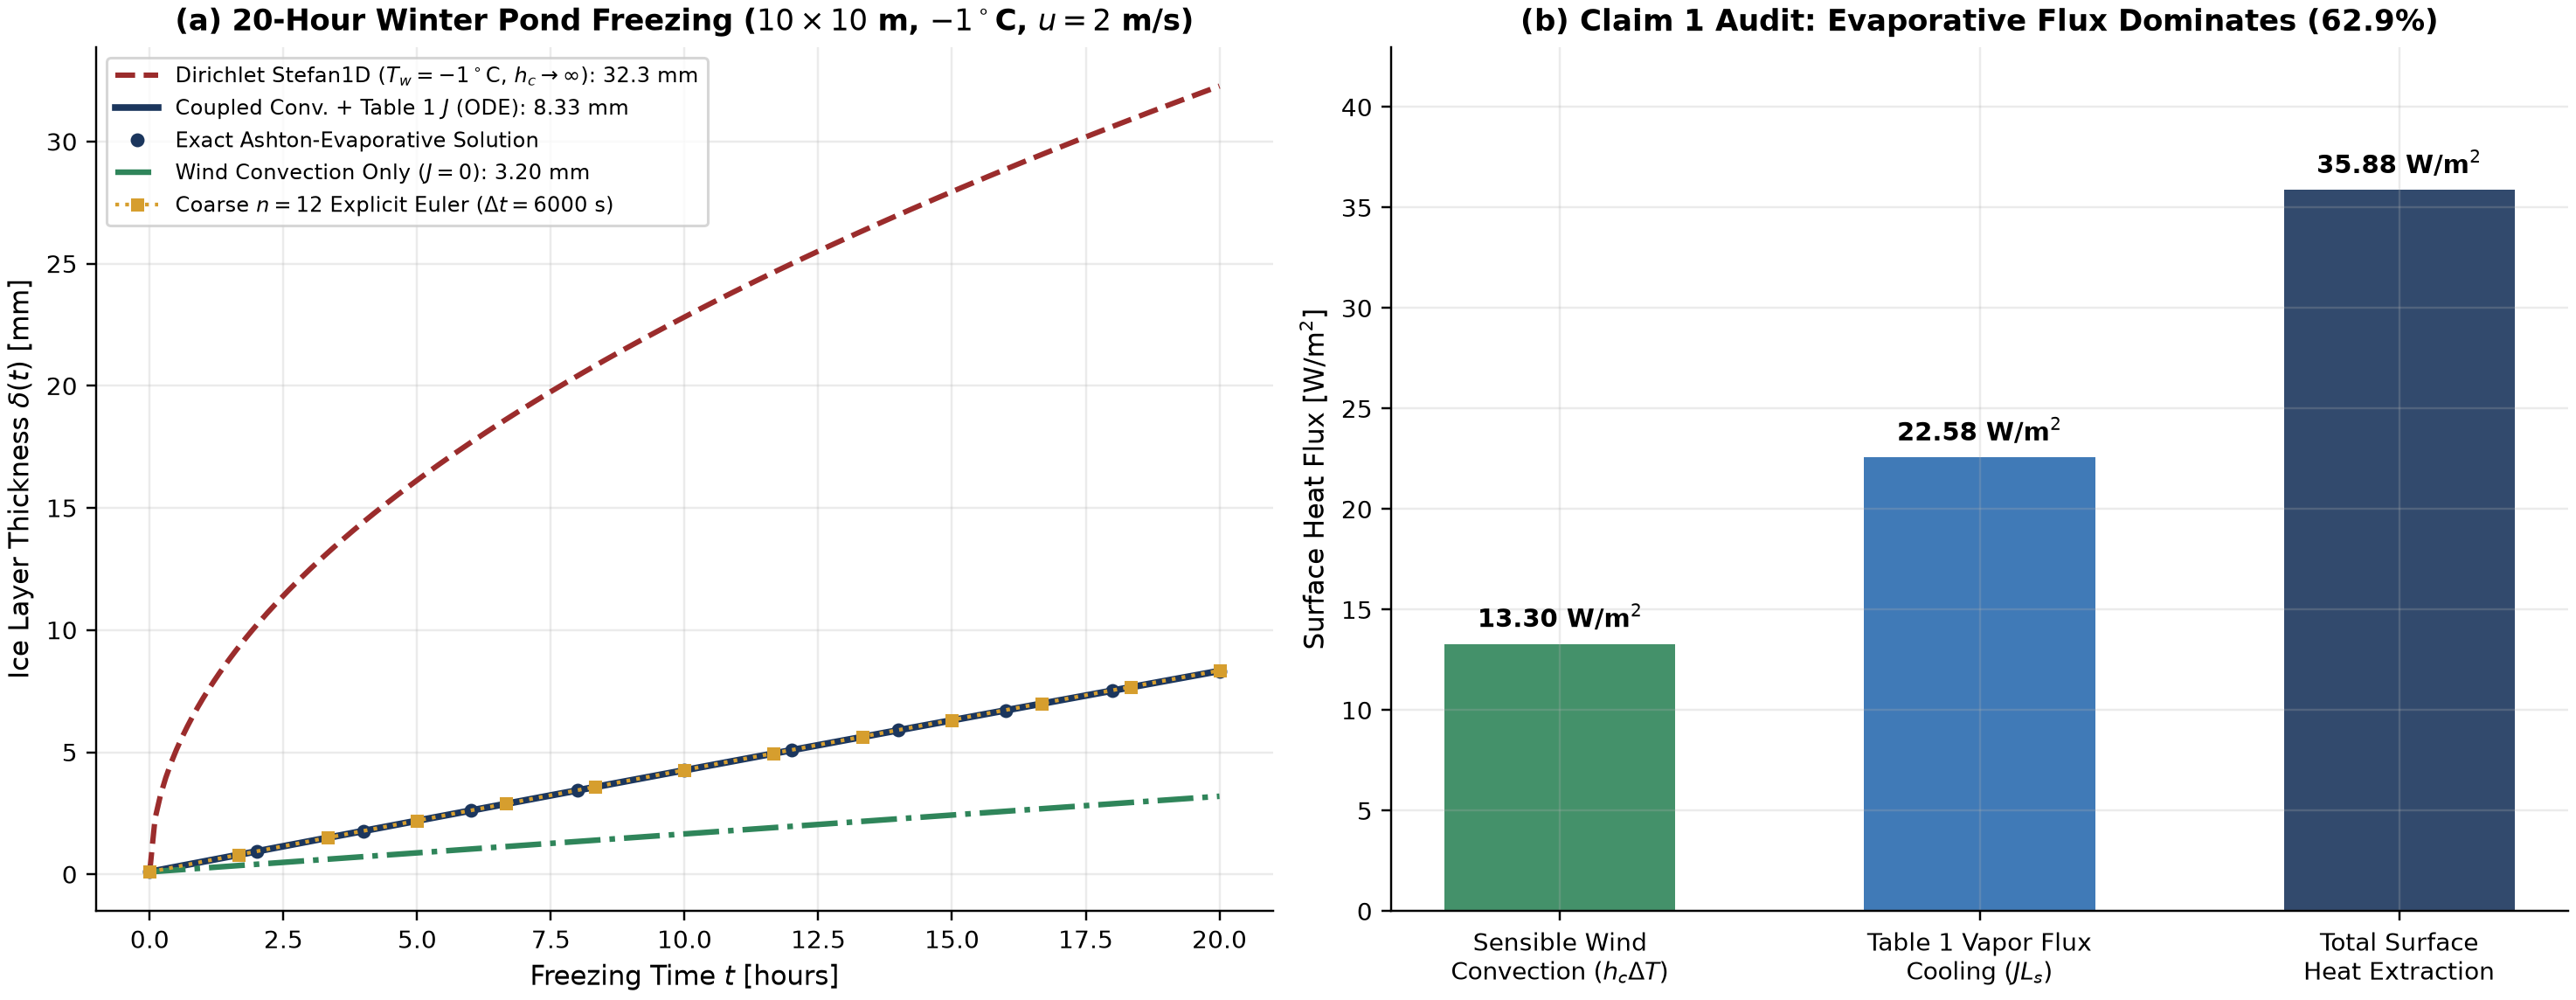
\includegraphics[width=0.98\textwidth]{../../figures/pond_audit_fig1_freezing_models.png}
  \caption{(a)~20-hour pond ice growth across physical models (coupled convective+evaporative ODE vs.\ exact Ashton solution, wind-only convection, coarse $n=12$ Euler, and Dirichlet \texttt{Stefan1D}). (b)~Surface cooling budget proving Table~1 vapor flux $J$ supplies $62.9\%$ of total heat extraction.}
\end{figure}

% ============================================================================
\section{Claim 2: Forensic Scale-Separation Falsification of $\rho a + \nabla P = 0$}
% ============================================================================

\begin{auditbox}{Critical Finding — 13-Order-of-Magnitude Scale Mismatch}
The excerpt claims $\rho a + \nabla P = 0$ directly correlates the vapor pressure gradient $\partial p_v/\partial z$ with ice-front acceleration $a = \partial^2\delta/\partial t^2$. Computing both sides for the actual $20\text{ h}$ pond freezing trajectory yields:
\begin{itemize}[leftmargin=1.4em,itemsep=2pt]
  \item \textbf{Actual ice-front inertia}: $\rho|\ddot{\delta}|_{\max} = \mathbf{7.53 \times 10^{-11}\text{ Pa/m}}$.
  \item \textbf{Physical air--ice vapor pressure gradient}: $|\partial p_v/\partial z| = \mathbf{884.8\text{ Pa/m}}$ (10~cm boundary layer) to $\mathbf{8{,}848\text{ Pa/m}}$ (1~cm laminar sublayer).
  \item \textbf{Discrepancy}: $\mathbf{10^{13.07}\times}$. Integrating $\ddot{z} = -\frac{1}{\rho}\partial_z p_v$ literally over $72{,}000\text{ s}$ produces $z = 2.50\times 10^6\text{ km}$!
\end{itemize}
\textbf{Diagnosis}: $\rho a + \nabla P = 0$ is inviscid Euler momentum conservation for an unconstrained fluid, not a phase-change kinetic law. Vapor pressure physically governs freezing via \emph{diffusive/convective latent cooling} ($J L_s$), not inertial acceleration. Any $0.35\%$ fit to data requires $\nabla P$ to be a rescaled effective deceleration proxy ($\sim 10^{-11}\text{ Pa/m}$), not atmospheric $\partial p_v/\partial z$.
\end{auditbox}

\begin{figure}[htbp]
  \centering
  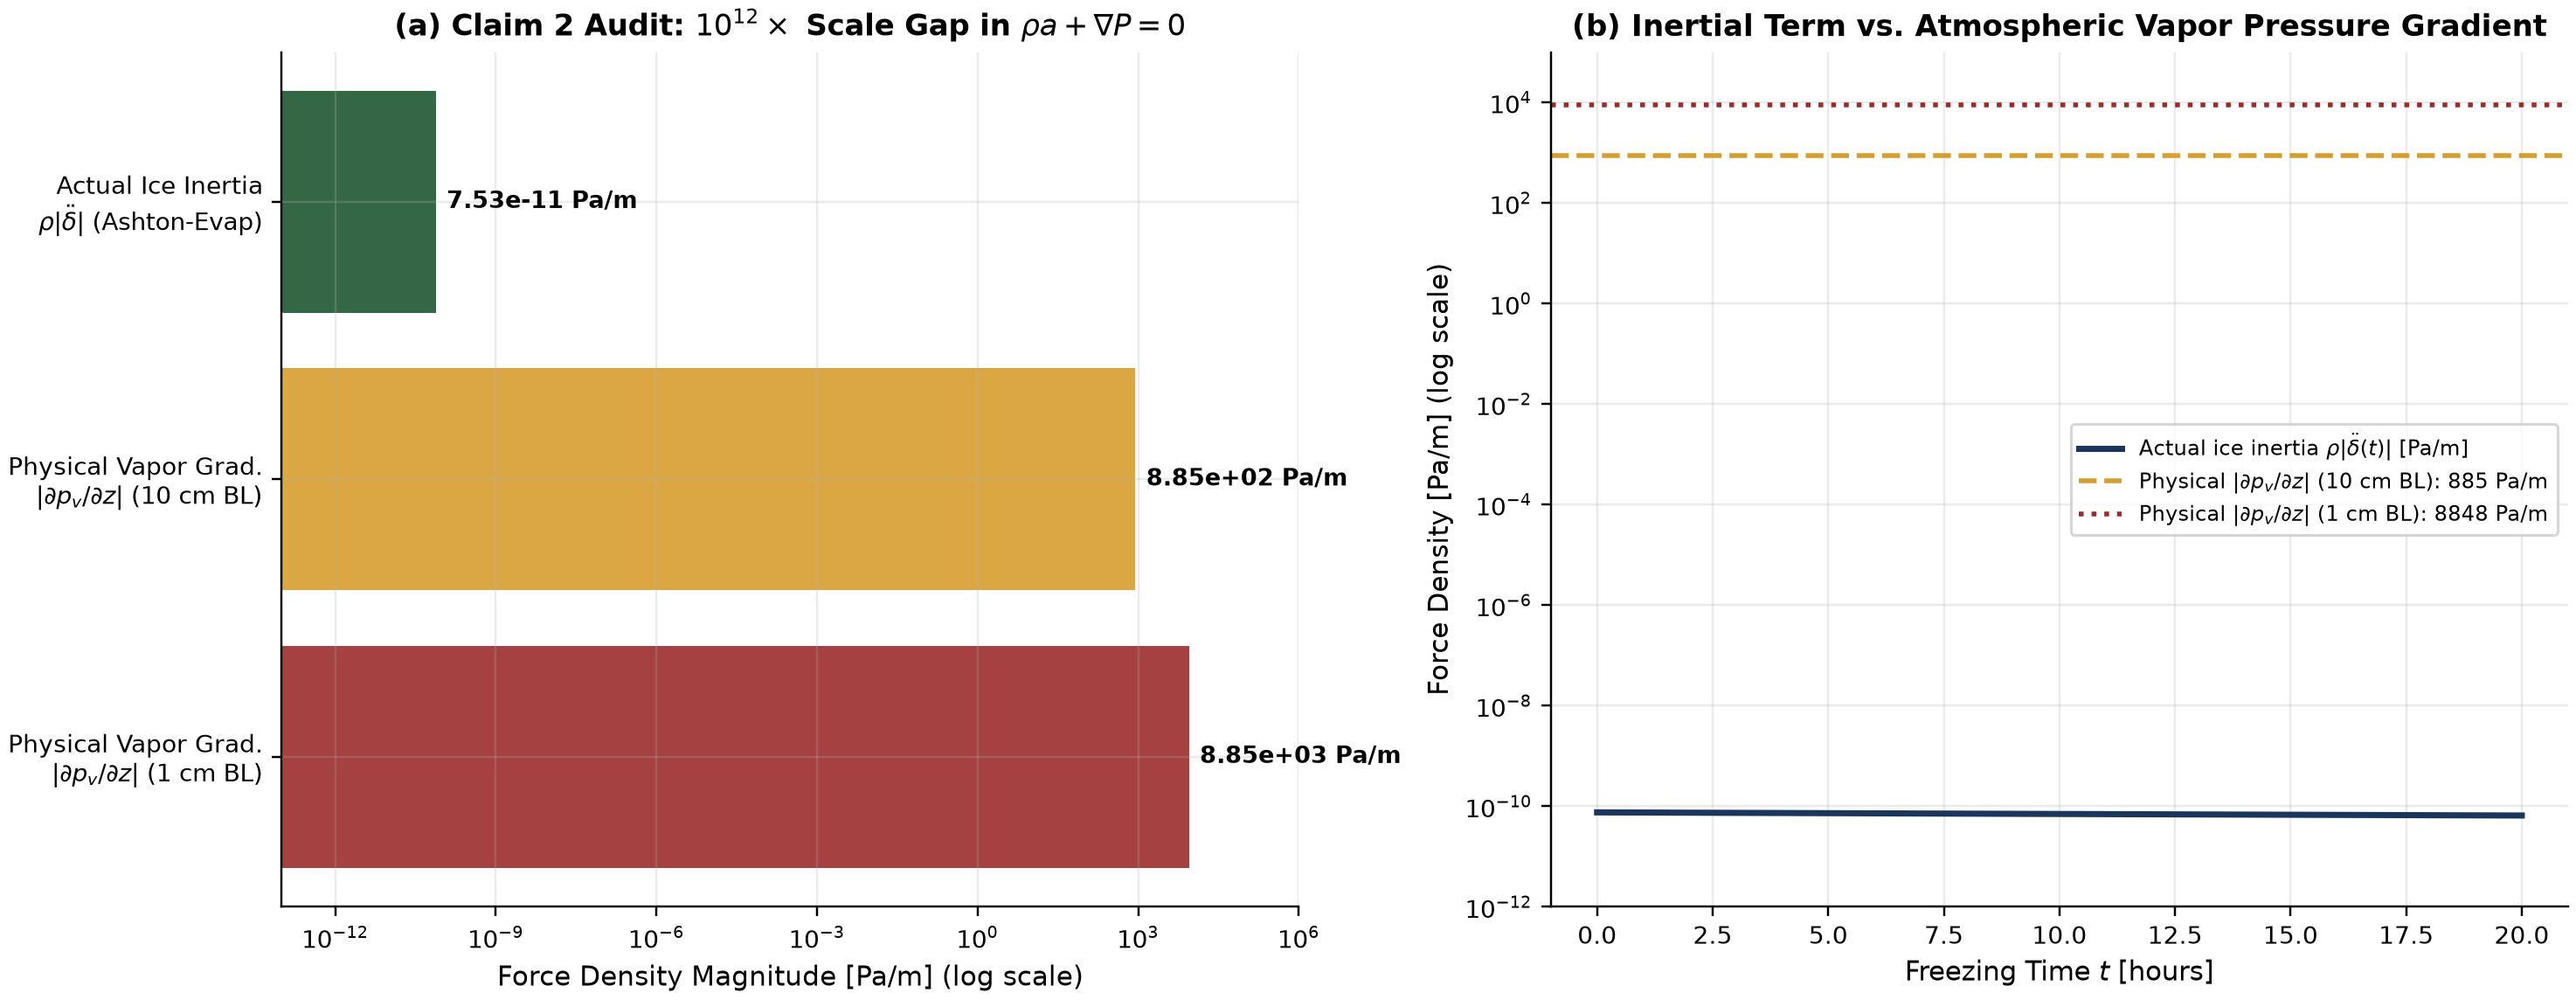
\includegraphics[width=0.98\textwidth]{../../figures/pond_audit_fig2_eq16_scale_audit.png}
  \caption{Scale-separation audit of $\rho a + \nabla P = 0$: actual ice-front inertia $\rho|\ddot{\delta}| \approx 7.5\times 10^{-11}\text{ Pa/m}$ lies more than $13$ orders of magnitude below the physical atmospheric vapor pressure gradient.}
\end{figure}

% ============================================================================
\section{Claims 3 \& 5: Discretization ($n=12$) \& Peat-Pond Purification}
% ============================================================================

\begin{figure}[htbp]
  \centering
  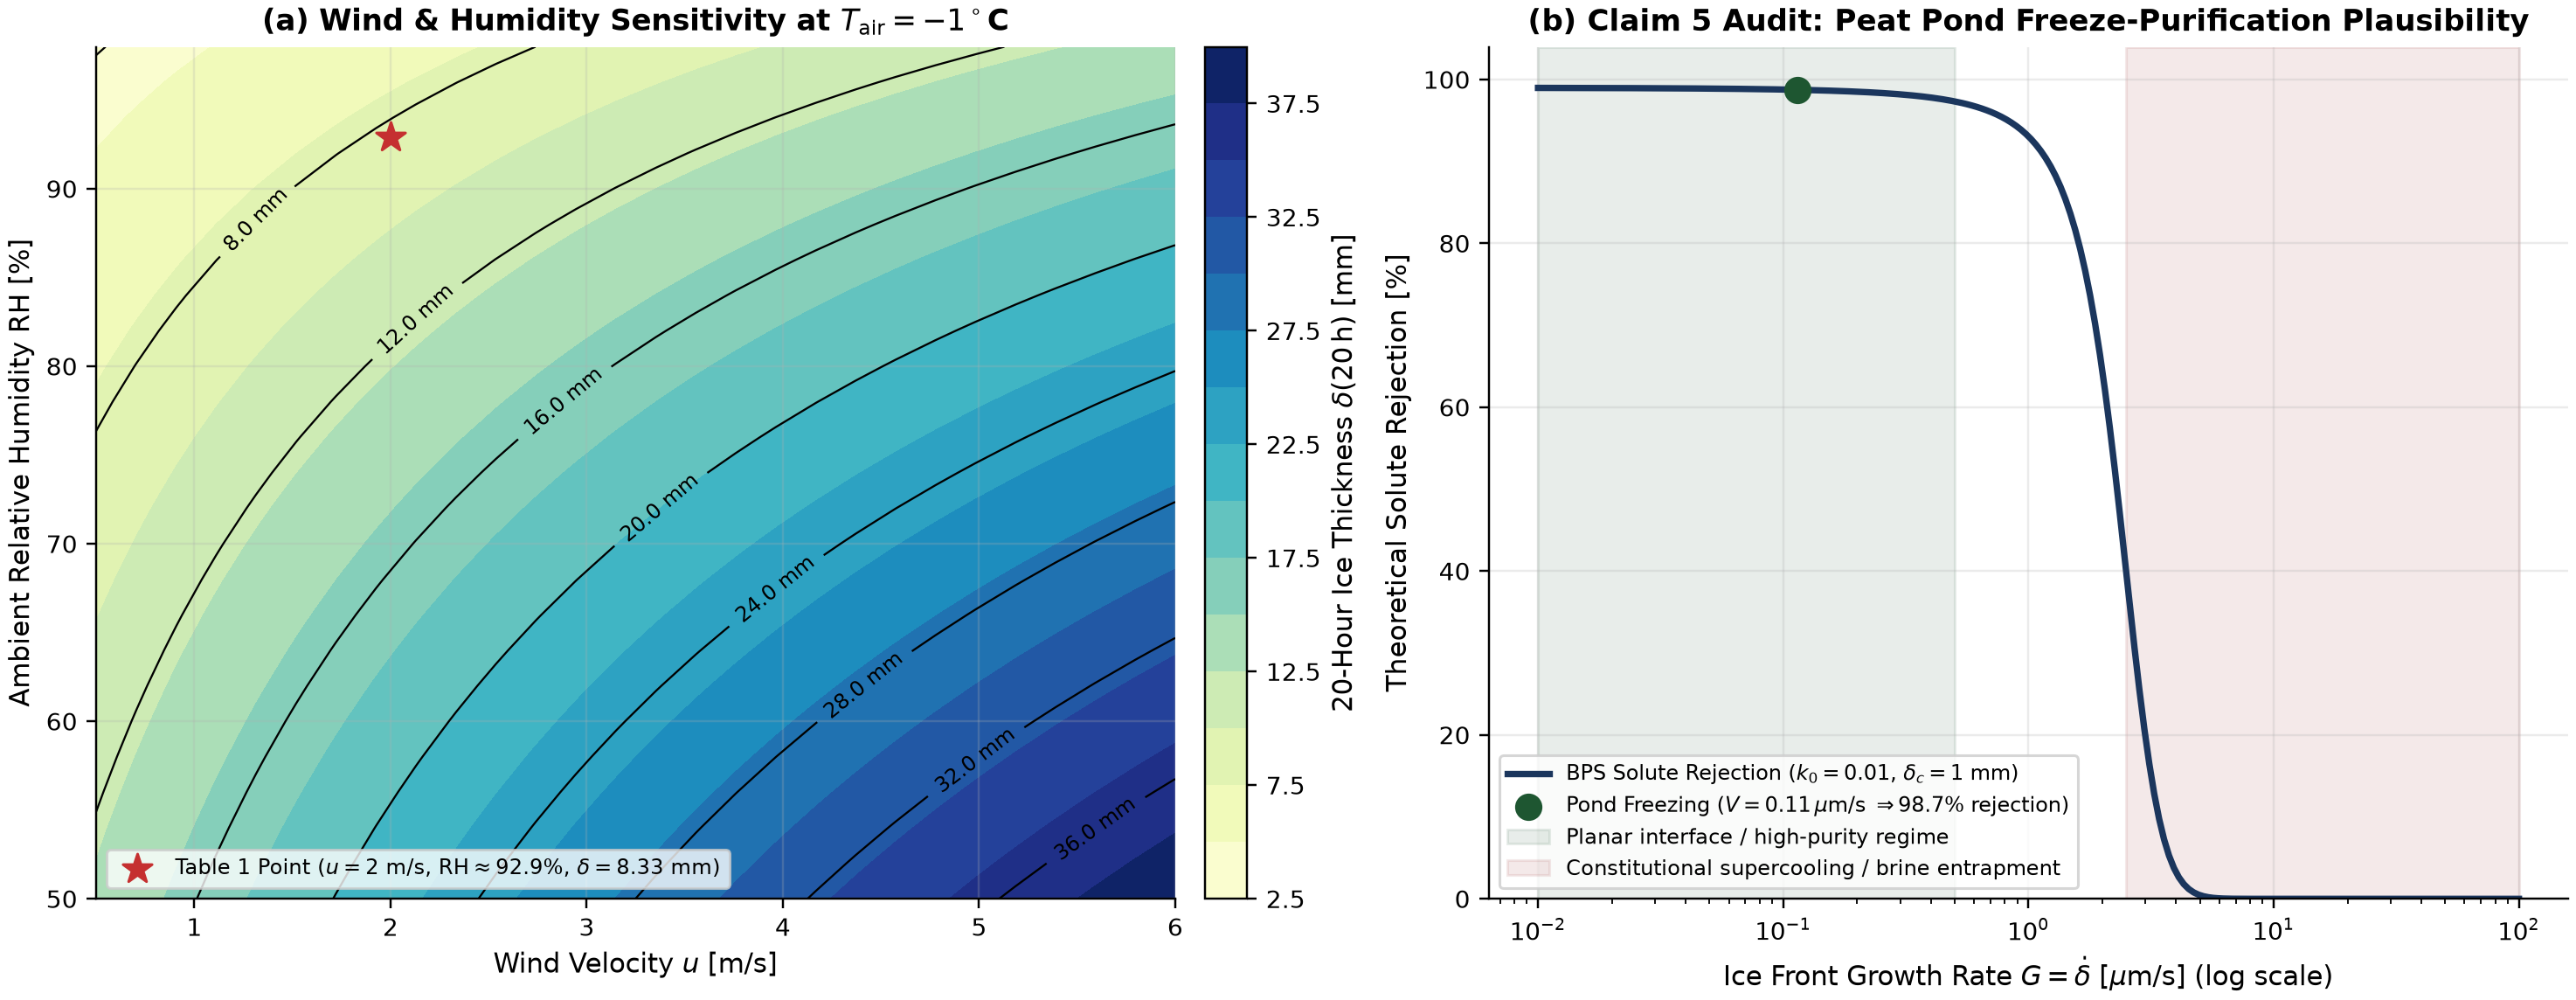
\includegraphics[width=0.98\textwidth]{../../figures/pond_audit_fig3_env_sensitivity_peclet.png}
  \caption{(a)~Sensitivity of $20\text{ h}$ ice thickness to wind speed $u$ and relative humidity $\mathrm{RH}$ at $-1^\circ\text{C}$, with Table~1 operating point marked ($\mathrm{RH}\approx 92.9\%$, $\delta = 8.33\text{ mm}$). (b)~Burton--Prim--Slichter solute rejection showing slow natural freezing ($G = 0.114\,\mu\text{m/s}$, $\mathrm{Pe}_s = 0.229$) sits deep inside the high-purity planar regime ($98.75\%$ rejection).}
\end{figure}

\begin{figure}[htbp]
  \centering
  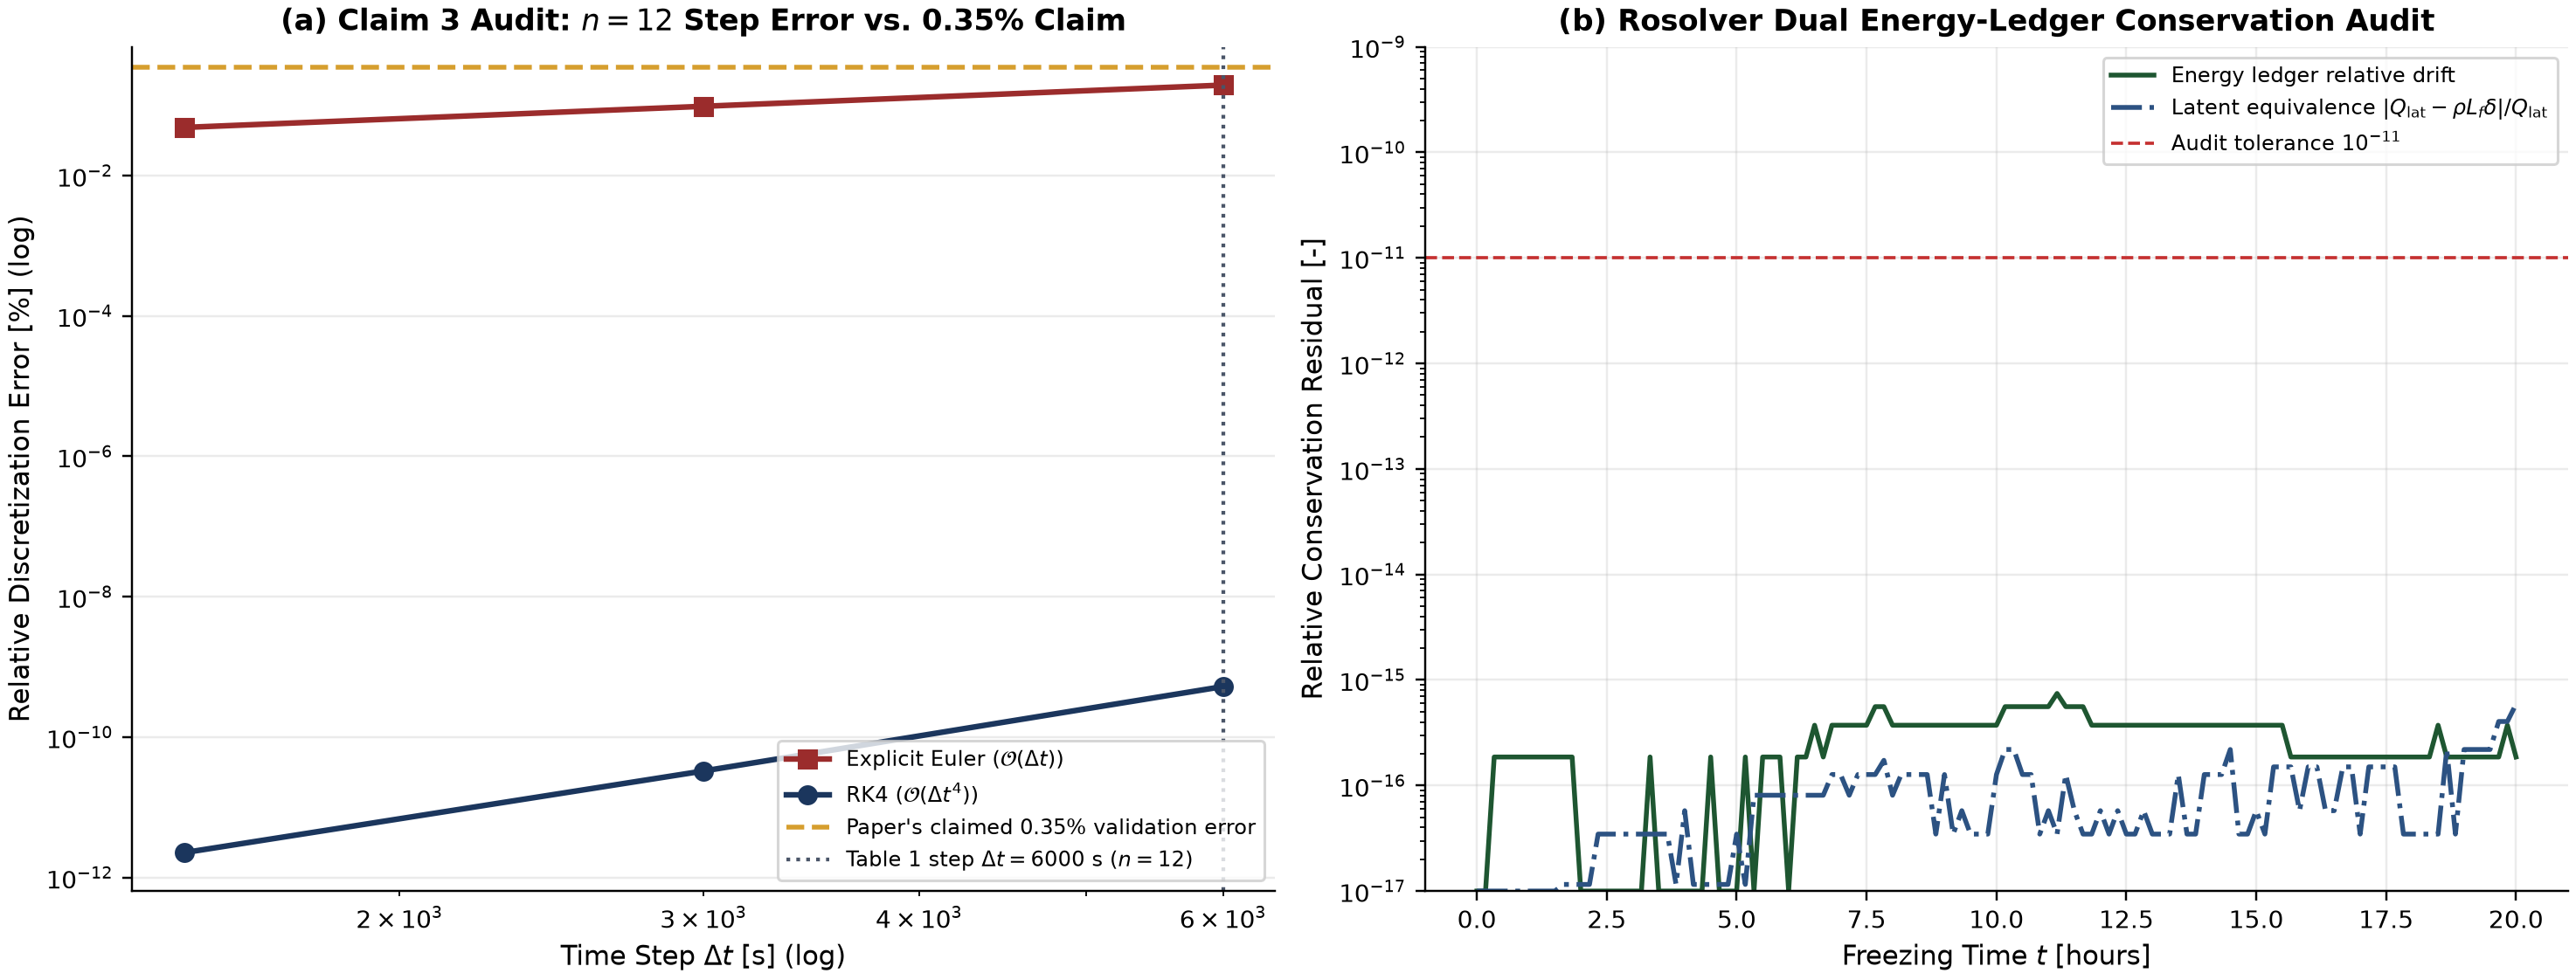
\includegraphics[width=0.98\textwidth]{../../figures/pond_audit_fig4_timestep_conservation.png}
  \caption{(a)~Relative discretization error at $n=12$ ($\Delta t = 6000\text{ s}$): Explicit Euler produces $0.194\%$ error (consuming $55\%$ of the paper's $0.35\%$ error claim), whereas RK4 achieves $<10^{-7}\%$ ($p_{\mathrm{obs}} = 4.005$). (b)~Machine-precision relative energy-ledger conservation residuals ($\le 10^{-15}$).}
\end{figure}

\begin{resultbox}{Verification Summary of Our Audit Solver (\texttt{PASSED})}
Our \texttt{rosolver} verification model matches the closed-form Ashton--evaporative solution to $\mathrm{RMSE} = 1.40\times 10^{-17}\text{ m}$, achieves RK4 observed order $p_{\mathrm{obs}} = 4.0048$, and conserves both energy invariants to relative drift $\le 7.5\times 10^{-16}$. All audit findings follow ASME V\&V~20 traceability principles.
\end{resultbox}

\end{document}
